%%%%%%%%%%%%%%%%%%%%%%%%%%%%%%%%%%%%%%%%%%%%%%%%%%%
%
%  New template code for TAMU Theses and Dissertations starting Fall 2012.  
%  For more info about this template or the 
%  TAMU LaTeX User's Group, see http://www.howdy.me/.
%
%  Author: Wendy Lynn Turner 
%	 Version 1.0 
%  Last updated 8/5/2012
%
%%%%%%%%%%%%%%%%%%%%%%%%%%%%%%%%%%%%%%%%%%%%%%%%%%%

%%%%%%%%%%%%%%%%%%%%%%%%%%%%%%%%%%%%%%%%%%%%%%%%%%%%%%%%%%%%%%%%%%%%%%
%%                           SECTION I
%%%%%%%%%%%%%%%%%%%%%%%%%%%%%%%%%%%%%%%%%%%%%%%%%%%%%%%%%%%%%%%%%%%%%


\pagestyle{plain} % No headers, just page numbers
\pagenumbering{arabic} % Arabic numerals
\setcounter{page}{1}


\chapter{\uppercase {Introduction}}

\section{Motivation}
Proliferation of smartphones and tablets is introducing a divide in the computer industry. While mobile technology is burgeoning in the role of access points, computationally intensive tasks are offloaded to the cloud \cite{virt_benefits}. As a result, the server industry is growing at a tremendous pace. This has also led to the development of associated technologies, the most prominent being virtualization \cite{virt_back}.

Virtualization enables multiple operating system environments to run simultaneously on one hardware platform. It provides added security and isolation in the form of an additional software layer below the OS (Operating System), called the hypervisor \cite{virt_arch}. This technology has become an industry standard for large server farms. Fault isolation, centralized control, workload balance, and live migration of machines are few of its many benefits \cite{virt_back}.

Most virtualized systems today, are constrained by memory and I/O subsystems \cite{virt_io_bottleneck} \cite{virt_bottleneck} \cite{virt_io_bottleneck2}, with CPU resources to spare. However, these limitations will no longer remain relevant with the upcoming radical changes in memory technologies. In the past few decades, memory subsystem structure has been fairly consistent, with revisions just in terms of size. However, new developments such as 3D memory stacks \cite{mem_3d1} \cite{mem_3d2}, Storage Class Memory \cite{scm1} \cite{scm2}, etc., will completely revolutionize memory architectures.

Among these new technologies, Non-Volatile RAM (Random Access Memory) in the form of SCM (Storage Class Memory), has the potential to overhaul memory architecture in virtual machines. Introduction of non-volatile memory can reduce the frequency of disk I/O operations, and diminish memory footprint of disk caches. It is highly likely that persistent memory will play a dominant role in future server farms. Thus, it is a natural and worthwhile initiative to inspect the possibility of sharing such a resource in virtual machines, with significant opportunities for performance gains in filesystems, boot procedures, crash recovery, etc \cite{nvm_benefits1} \cite{nvm_benefits2}. This thesis is going to focus on some of these aspects. To the best of our knowledge, there has been no prior work in this direction, and this work can be considered as a first step in enabling NVRAM (Non-Volatile RAM) sharing in virtualized environments 

\section{Overview}

This work focusses on sharing non-volatile memory in virtualized environments. Due to several contrasting properties between volatile and non-volatile memory, a conventional Memory Management Unit (MMU) cannot be used to manage non-volatile memory. Therefore, a novel design of an additional MMU is proposed to facilitate non-volatile memory sharing. This thesis also showcases an implementation of the non-volatile MMU in a popular open source hypervisor -- Xen, along with detail on its performance metrics and directions of future work.

In Chapter 1, we provide a brief technical background of virtualization and memory subsystem in a modern computer. Chapter 2 is dedicated to the internal architecture of Xen, detailing its subcomponents and various design philosophies. In Chapter 3, we discuss the design and implementation details of the non-volatile MMU. In Chapter 4, we present the specifics of the experimental setup along with the results. Lastly, in Chapter 5, the merits and demerits of the system are discussed with emphasis on future work. 

\section{Virtualization}
Modern day computers are a combination of complex software and hardware systems. Such a high level of engineering is made possible through concepts of abstraction, where an upper layer interacts with the layer beneath it, using well defined interfaces, oblivious to the lower layer's inner implementation complexity and details.

A computer system can be viewed as a stack of several independent layers as shown in Fig \ref{fig:appstack}. Here the flexibility of each layer is constrained by the interfaces defined both above and below it. 

\setlength{\belowcaptionskip}{-10pt}

\begin{figure}[H]
  \centering
  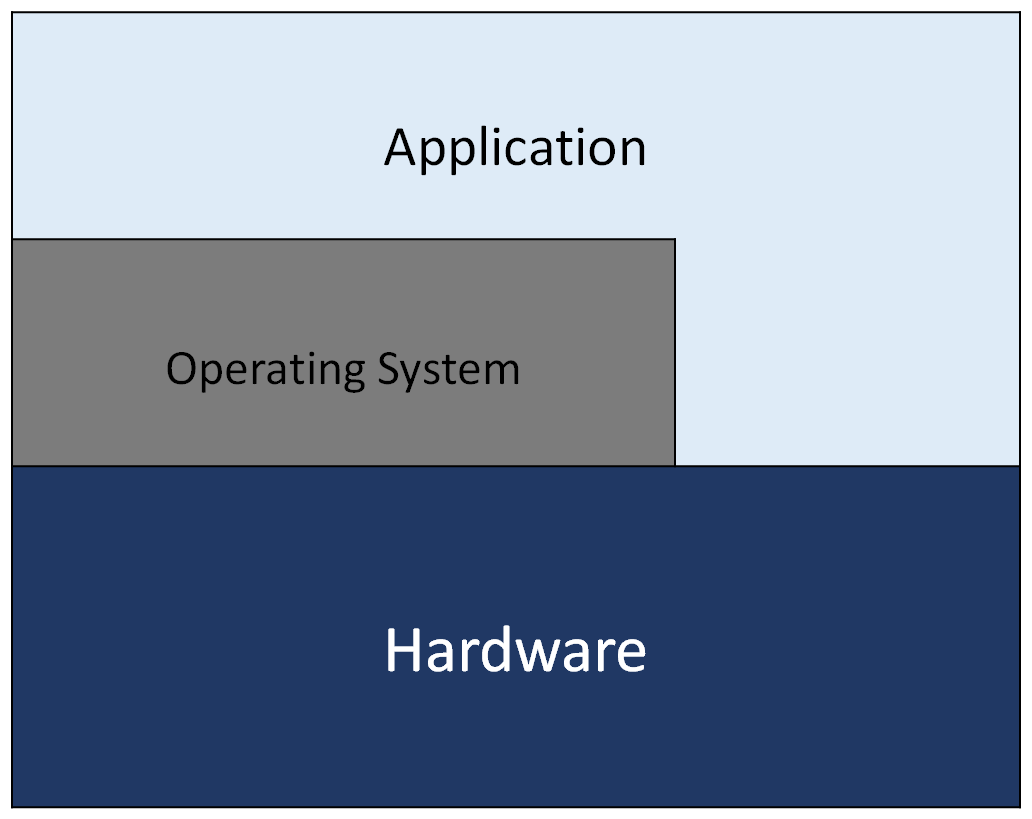
\includegraphics[scale=0.6]{figures/app_stack.png}
  \caption{Conventional Application Stack}
  \label{fig:appstack}
\end{figure}

Virtualization provides a way to relax the above constraints, either in the form of the entire system or a subsystem like memory, I/O processor etc. It enables the mapping of a virtual system, to real system resources thereby giving an illusion to the process/OS of a custom virtual environment, different from the host machine \cite{virt_arch}.

Formally, virtualization can be defined as a mapping between a guest state ($S_i$) and a host state ($S'_i$), such that a sequence of operations, $e_k$, modifying the guest state from ($S_i$) to ($S_j$), can be represented by some corresponding sequence of operations, $e'_k$, which modifies the host state from ($S'_i$) to ($S'_j$) respectively \cite{smith_nair}. 

\setlength{\belowcaptionskip}{-10pt}

\begin{figure}[H]
  \centering
  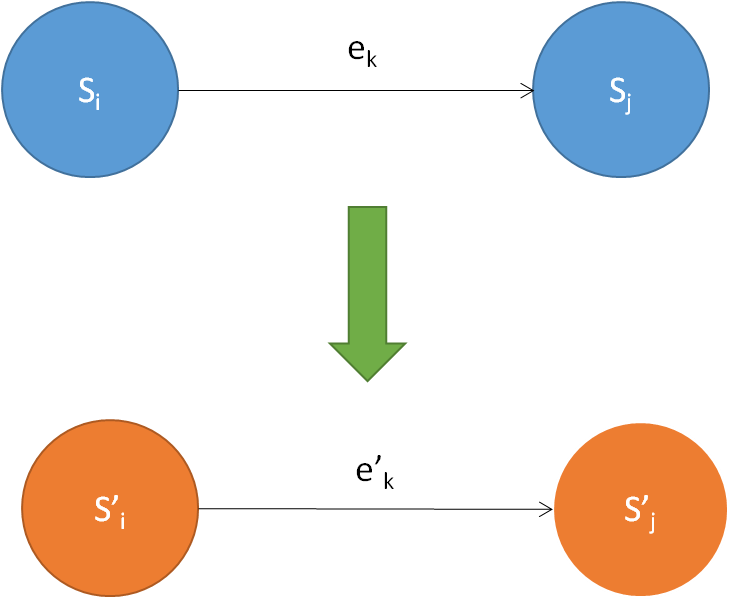
\includegraphics[scale=0.8]{figures/vir_phy_map.png}
  \caption[Equivalent State Mapping]{Equivalent State Mapping \cite{smith_nair}}
  \label{fig:statemap}
\end{figure}

From an OS's point of view, all hardware can be classified into three broad categories.

1. CPU: A CPU is a highly complex piece of hardware abstracted for the OS in the form of an Instruction Set Architecture (ISA). The ISA defines the actual hardware software interface in a machine, converting software code into electrical signals which percolate through the entire system. Every action performed by the software stack (including controlling Memory and I/O) takes place through the available set of ISA instructions.

2. Memory: Memory is a collection of byte-addressable memory elements which can be used to store and retrieve data. Every ISA provides special instructions to interact with memory.

3. I/O: All devices apart from CPU and Memory, such as modem, printer, monitor, etc., come under the category of I/O devices. These devices are essentially composed of several specialized registers which can be programmed to perform device specific instructions. Thus from the CPU’s perspective, there is not much of a difference between I/O and memory, since both are collection of byte addressable memory elements. Interactions with an I/O device can be performed by either (optional) special I/O instructions or standard memory instructions supported by the ISA. Due to the vast variety of devices available from different manufacturers, individual device drivers have to be developed and added to the OS separately.

\setlength{\belowcaptionskip}{-10pt}

\begin{figure}[H]
  \centering
  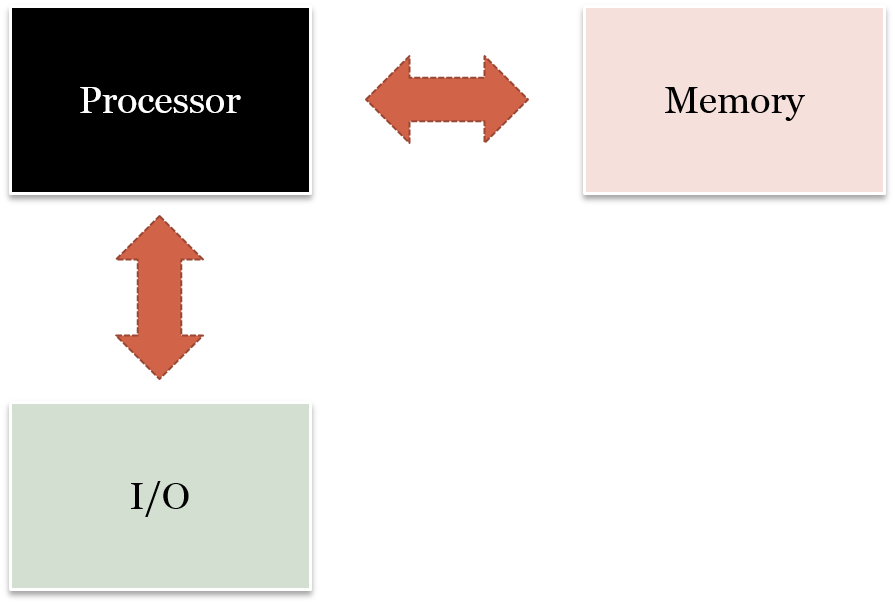
\includegraphics[scale=0.8]{figures/Mem_IO_CPU.png}
  \caption{Abstract Computer Model}
  \label{fig:mem_io}
\end{figure}
For entire system virtualization, we have to virtualize all the subsystems. This can be performed either in software, or by hardware. A software approach provides higher flexibility at the cost of reduced performance when compared to a hardware solution. The following subsections delve further into each subsystem virtualization specifics.

\subsection{CPU Virtualization}
CPU virtualization aims at providing the hypervisor direct control over the distribution of hardware resources amongst various VMs (Virtual Machines). Work of similar nature is performed at the application layer by the Operating System. To facilitate such protection mechanisms, a typical ISA implements several privilege levels (protection rings), allowing a certain class of instructions to execute only in a privileged mode. The ISA generally presents two levels -- user level and supervisor level. An attempt to execute a privileged instruction in an unprivileged mode triggers an exception. It transfers control of execution to a specific supervisor level subroutine (generally registered with the OS), which takes appropriate action maintaining the security and protection of the system.

\setlength{\belowcaptionskip}{-10pt}

\begin{figure}[H]
  \centering
  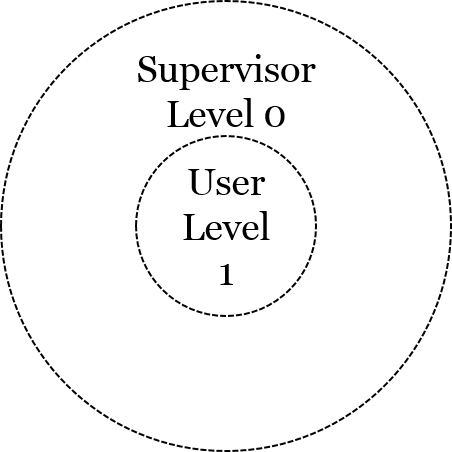
\includegraphics[scale=0.6]{figures/protect_levels.png}
  \caption{ISA Protection Rings}
  \label{fig:protect_2}
\end{figure}
In the case of virtual machines, such a task becomes all the more challenging, as these protection mechanisms have to be implemented at the OS level by the hypervisor. Pioneering work done by Popek and Goldberg \cite{popek}, defined several constraints on the Instruction Set Architecture of a machine to provide efficient virtualization where majority of the operations run naively on the CPU ISA instructions. The CPU instructions are first classified in the following manner:

1. Privileged Instructions: The group of instructions that can only be run when the CPU is in supervisor mode, and will trap outside it.

2. Control Sensitive Instructions: Instructions that change the hardware configuration or resources of the system.

3. Behavior Sensitive Instructions: Any instruction whose output depends upon the current state, or configuration of the machine.

They proposed that for any architecture to be efficiently virtualizable (in trap and emulate model), all sensitive (behavior and control) instructions must be privileged instructions. Any instruction, which either tries to modify hardware configuration, or whose output depends upon it, should transfer control of execution to the hypervisor.

Contrary to norm, an operating system on a VM runs in de-privileged user mode. Most of the operations run at native speeds without emulation, with a penalty introduced for sensitive instructions which trap into the hypervisor.

\setlength{\belowcaptionskip}{-10pt}

\begin{figure}[H]
  \centering
  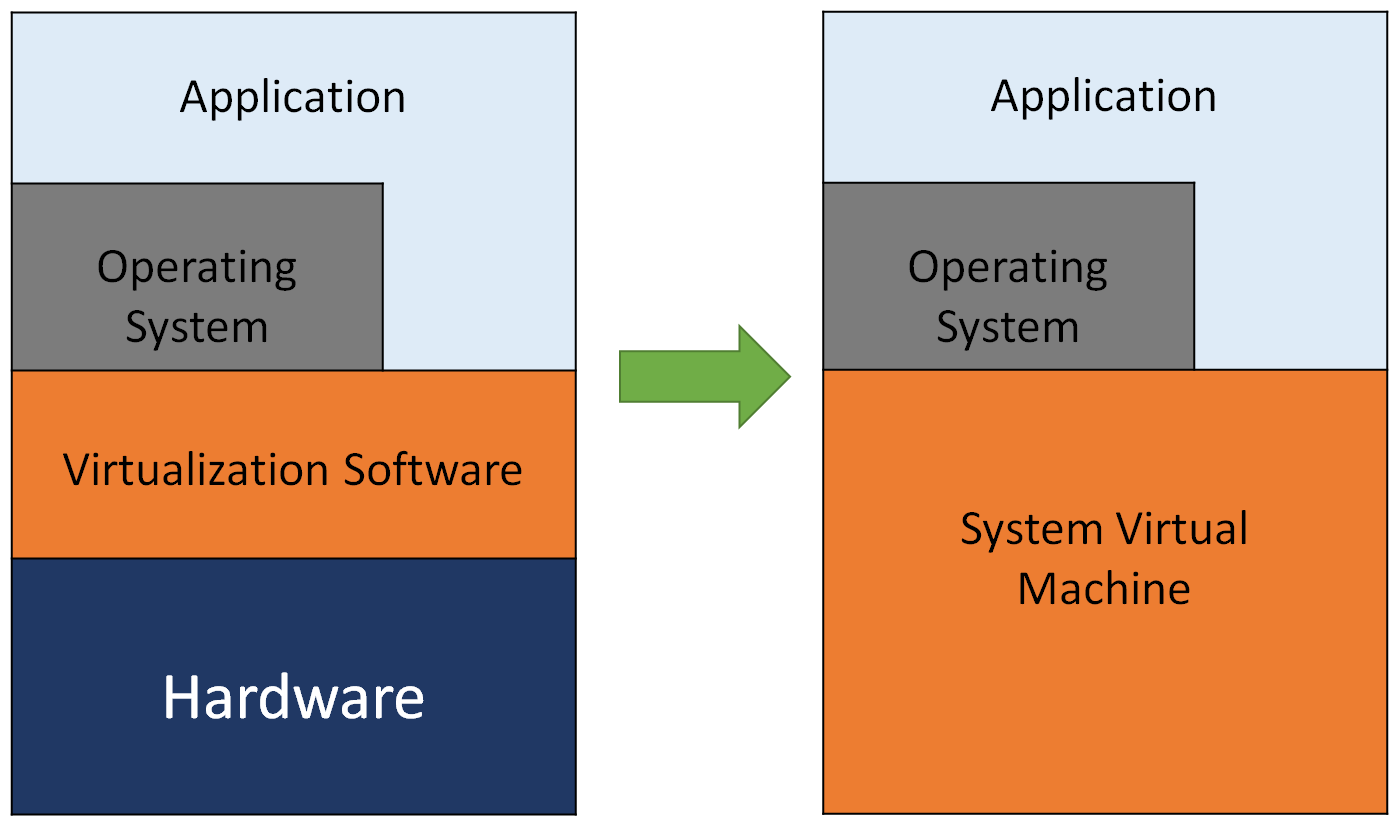
\includegraphics[scale=0.6]{figures/sys_virt.png}
  \caption{System Virtualization Model}
  \label{fig:sys_virt}
\end{figure}

According to the above definition, x86 is not a virtualizable architecture. It has a set of 17 sensitive instructions which do not trap to the supervisor mode. Being a predominant architecture in today’s computers, significant efforts have been spent producing several solutions.

1. Emulation is the most versatile solution, implemented entirely in software. Here, the dynamic instruction stream is scanned for sensitive instructions, which are then replaced by emulated operations. Emulation can also allow a code, compiled for one ISA, to run on a host machine with a different ISA; though with a severe performance penalty (since every instruction has to be emulated). Binary translation can be viewed as an optimized version of the above, where emulated code segments are cached aggressively, providing significant performance boost for re-entrant code segments.

2. Paravirtualization is another solution, which relies on relaxing some of the tenets of virtualization by modifying the source code of operating system to replace sensitive operations with hypercalls to the hypervisor. Unfortunately this trades off flexibility with performance, as different Operating Systems have to be modified individually and the OS source code may not be available to the hypervisor. Xen is one of the leading open-source hypervisors employing paravirtualization \cite{xen_virt}, now natively supported by the Linux kernel (from Linux kernel 3.0 onwards).

3. With increasing demand for virtualization technology both Intel and AMD have extended the x86 ISA to include extra features to support a hypervisor in an additional ring at -1 level. As per the original requirements of Popek and Goldberg, the OS executing in the ring 0 is oblivious to the presence of the hypervisor, with the privileged instructions generating a trap to the hypervisor. Additional level of memory virtualization is also introduced with the addition of Extended Page Tables in hardware. Along with the above, several instructions were added to the ISA to support a system call structure for the hypervisor, named hypercalls. It also provides a hardware concept of virtual CPUs with specific instructions to store/restore the state to/from VMCS (Virtual Machine Control Structure). This enables x86 to achieve the status of a virtualizable architecture with the support of these extensions. Detailed explanation is provided in Section 1.5. 

\setlength{\belowcaptionskip}{-10pt}

\begin{figure}[H]
  \centering
  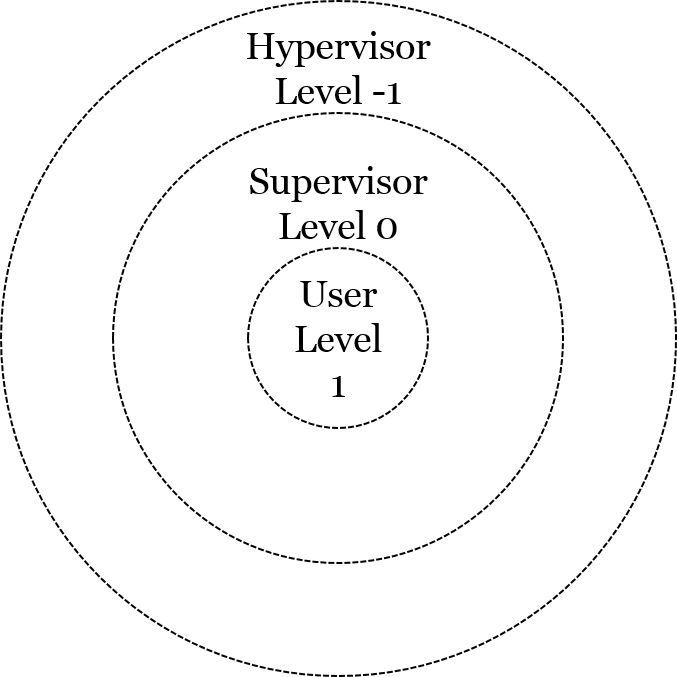
\includegraphics[scale=0.6]{figures/protect_hyper.png}
  \caption{Hypervisor Protection Rings}
  \label{fig:hyper_rings}
\end{figure}

\subsection{Memory Virtualization}
Virtual Memory has been around for a long time, allowing multiple applications to share the physical memory in the system. Each application is given a virtual address space, which is mapped on to the available physical address space via page tables maintained by the Operating System. Thus applications do not have to worry about runtime memory allocation, and can operate on a continuous address space. On the downside, each memory reference now requires an address translation through the page table structure. Many ISA’s provide support for a hardware page table walker, which performs the translation in hardware. 

\setlength{\belowcaptionskip}{-10pt}

\begin{figure}[H]
  \centering
  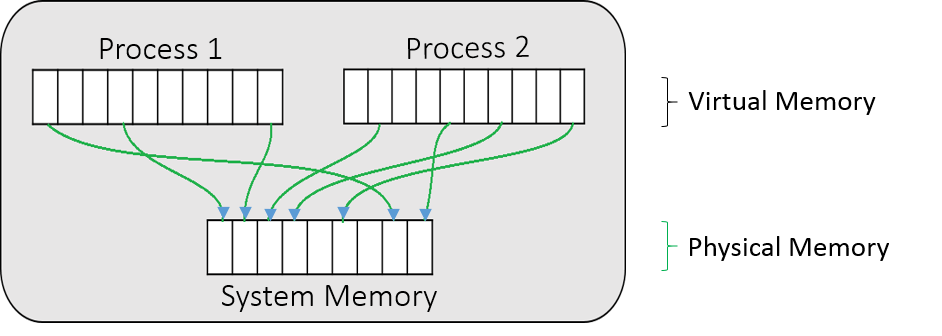
\includegraphics[scale=0.8]{figures/virt_mem.png}
  \caption{Virtual Memory}
  \label{fig:virt_mem}
\end{figure}
In a virtualized environment the system memory is shared among several guest VMs. Thus it leads to an additional address space.

1. Virtual address space: The address space as visible to applications.

2. Guest Physical address space: Individual VM Level or OS Level address space.

3. Real or Machine address space: The actual system memory address space.

\setlength{\belowcaptionskip}{-10pt}

\begin{figure}[H]
  \centering
  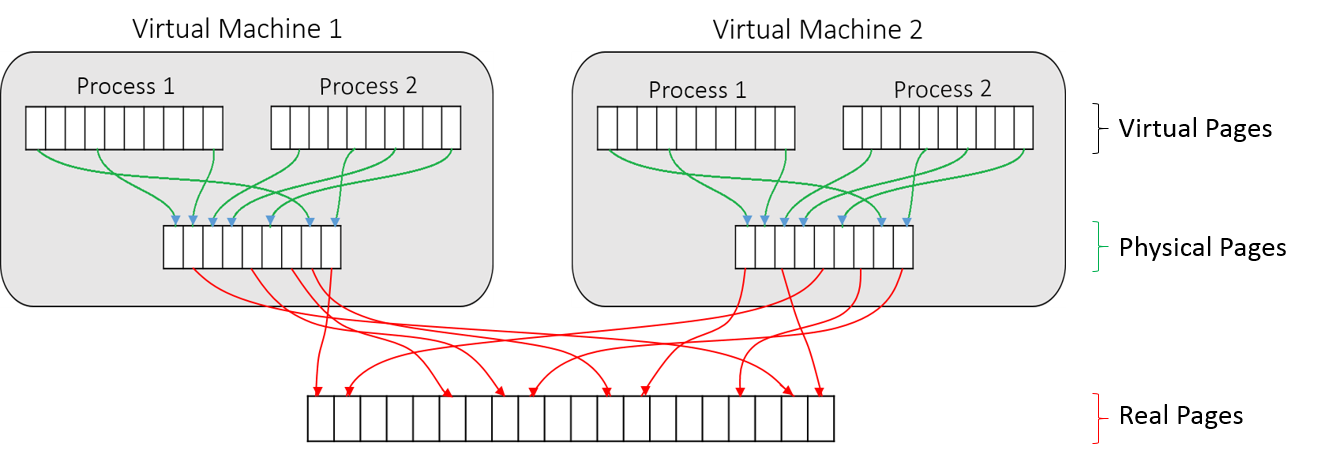
\includegraphics[scale=0.65]{figures/hyp_mem_map_comp.png}
  \caption{Hypervisor based Memory Layers}
  \label{fig:hyper_mem}
\end{figure}

Translations from virtual address space to the machine address space require two levels of paging:

1. Operating System Page table: Translates from virtual to guest physical addresses.

2. Hypervisor Page table: Translates from guest physical to machine addresses.

Without additional hardware support, a clever software based solution is to maintain an additional shadow page table with the hypervisor, mapping virtual addresses directly to machine addresses. This approach though avoids one level of paging, causes frequent traps to the hypervisor, which are very expensive.

However, recent virtualization extensions added to the x86 architecture now support nested page tables, i.e. two levels of address translations in hardware. It provides far superior performance as compared to the shadow page table approach. In the event of a page fault due to an invalid entry in the guest page tables, the hypervisor need not be involved. However, in the software based approach, the hypervisor first catches the exception and forwards the event to the guest kernel for an appropriate response. It results in two unnecessary context switches, which can be avoided with nested page table support, where the exception is directly delivered to the guest. Moreover, any update to the guest page tables in the former approach have to go through hypervisor, either via hypercalls or exceptions. As evident, the number of context switches keep multiplying for shadow page tables. On the downside, a TLB (Translation Lookaside Buffer) miss is quite expensive, as the hardware has to traverse higher number of page tables to resolve an address.

Frequent context switching is another common issue faced in virtualized systems. To reduce its impact, the virtualization extensions provide tagged TLB entries, where TLB entries are associated with a vCPU (virtual CPU) using a tag. Thus every context switch does not necessitate a complete TLB flush. It can be safely assumed from the above that hardware extensions add significant boost to most virtualized environments, especially for memory management.

\subsection{I/O Virtualization}
An I/O operation is typically controlled by programming special registers on the device, and using DMA (Direct Memory Access) for data transfers. Since device speeds are extremely slow (when compared to CPU) it is best not to involve the CPU. Thus DMA requests are moderated entirely by the northbridge chipset (see Fig \ref{fig:intel_arch}). The CPU is notified of the completion of the DMA operation, using an interrupt. Device virtualization mainly focusses on the following two aspects.

1. DMA

2. Interrupts

There are several ways to approach this problem. A direct method would be for the hypervisor to manage all the devices directly, and then emulate them for each Virtual Machine. It is a humungous undertaking requiring re-development of device drivers separately for the hypervisor. An alternate and currently popular way is to assign devices to specific privileged domains, which in turn, handle the I/O requests of all the other domains. Herein arises a security issue, where DMA requests from the driver domain can corrupt memory regions of other virtual machines. Traditionally there exists no security checks in hardware to prevent devices from accessing memory regions. As a result, the VM controlling a device, can potentially gain access to the entire machine address space.

Newer extensions such as VT-d (from Intel \cite{intelvtd}) can safeguard against such situations. VT-d implements IOMMU (I/O Memory Management Unit) which act as a MMU for devices. The hypervisor can program page tables in the IOMMU mapping the device to the guest physical address space of a particular VM, maintaining memory isolation for the other guests. Moreover VT-d also includes functionality for remapping interrupts to a particular virtual CPU construct. It helps minimize costly context switches and hypervisor interventions.

Newer ambitious approaches similar to PCI-e SR-IOV technology (Single Root I/O Virtualization) \cite{sriov}, define certain standards for a device to divide itself into smaller units. These smaller device units can then be directly controlled by individual VMs without hypervisor intervention. The hypervisor only maintains control of higher level functionality of the device, such as allocation of units to different VMs. Unfortunately, due to the vast number of devices and manufacturers involved, industry has not come to a common consensus, and the above approach is still in the nascent stages of development. 

\section{Non-Volatile Memory}
Traditionally a computer has two forms of data storage.

1. Main memory or RAM.

2. Secondary storage or Disk.

The key property of main memory is byte addressable data, while that of secondary storage is non-volatility -- data is preserved in the absence of power. Traditionally main memory has been volatile, while data on disk storage could only be accessed in blocks (~ 512 B to 4 KB). Moreover, disk is significantly slower and has enormous capacity in comparison to RAM (Table \ref{tab:sdd_ram_comp}). These factors have led RAM to serve as a cache for movement of data to and from disk.

\setlength{\belowcaptionskip}{-10pt}

\begin{table}[H]
  \centering
  \caption[Comparison between HDD, SSD and DRAM]{Comparison between HDD, SSD and DRAM (approx. values)}
  \label{tab:sdd_ram_comp}
  \begin{tabular}{|c|c|c|c|}
      \hline
      Property & HDD & SSD & DRAM \\
      \hline
      Maximum Capacity  & 6TB  & 512GB &  16GB\\
      \hline
      Data Retention &  $>$10 yrs &  10 yrs &  64ms  \\
      \hline
      Write Endurance &  Unlimited &  10000/block &  Unlimited \\
      \hline
      Read Latency & 3ms & 20us & 50ns     \\
      \hline
      Write Latency & 3ms & 200us & 50ns   \\
      \hline
      Cost (\$/GB) & 0.05 & 0.5 & 10        \\
      \hline
      Write Bandwidth & 150MB/s & 500MB/s & 10GB/s  \\
      \hline
  \end{tabular}
  %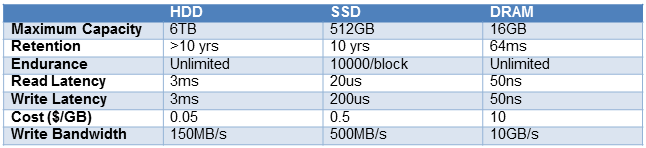
\includegraphics[scale=0.6]{figures/nvmemorytable.png}
\end{table}
The volatility of RAM leads to data loss on shutdown. In the case of a planned shutdown, data residing on RAM is backed up on the disk. The system state is restored on boot up by transferring all saved data back to RAM, generating an illusion of persistence of data. However, the heart of the problem lies in the case of unplanned power failures where all data present in the main memory is permanently lost. Several different approaches can be taken to safeguard against such a situation:

1. Software solution: -- This method cannot completely eliminate data losses, but tries to minimize the effective data loss. Here, the OS maintains complex data structures along with logging and check-pointing procedures to periodically transfer data to disk. Since disk speeds are significantly slower, heavy performance penalty is observed. The frequency of the above mentioned procedures involves a constant trade-off between performance and data integrity, where one has to be sacrificed for the other. This issue is exacerbated in server farms, where client data safety is of utmost importance.

2. Un-interruptible power source: -- This solution comes at steep infrastructure costs of a backup power source, which lies idle for the most part.

3. Hardware solution: -- Non-volatile RAM is a proposed hardware solution to the above mentioned issues. It combines near RAM access speeds with data retentive technologies to provide performance as well as data integrity. Data movement on the memory bus is several orders of magnitude faster when compared to disk, providing persistence at little or no additional cost.

Out of these three possibilities, the software solution is most commonly applied to current systems, due to the absence of an inexpensive alternative. Whereas, NVRAM technology, though in its nascent stages, is the most promising solution in the future systems. In conclusion, Non-Volatile memory is useful to safeguard against data loss during unexpected power cuts. 

\subsection{Storage Class Memory}

Research and innovation into devices has allowed a new class of memory technologies to spring up under the banner of Storage Class Memory which fall in the NVRAM category. Some common examples are PCM (Phase change memory) \cite{pcm}, STT-RAM (Spin Transfer Torque RAM) \cite{sttram}, ReRAM (Resistive RAM) \cite{reram1} \cite{reram2}, FRAM (Ferroelectric RAM) \cite{feram}, MRAM (Magnetic RAM) \cite{mram1} \cite{mram2}, etc. Each of these devices have different properties in terms of power efficiency, speed, density, and cost/bit, but are unified by the following common characteristics.

1. Byte Addressable Memory

2. Non-volatility

3. Significantly faster access times when compared to disks or SSDs.

Introduction of SCM will see a change in the motherboard architecture (Fig \ref{fig:new_arch}). It can be placed alongside DRAM on the memory bus, and also on a PCIe (Peripheral Component Interconnect Express) bus along with SSDs. With the growth and commercialization of different SCM technologies, SCM is expected to replace/augment both DRAM and Flash memory from their dominant roles in conventional machines in the near future. 

\setlength{\belowcaptionskip}{-10pt}

\begin{figure}[H]
  \centering
  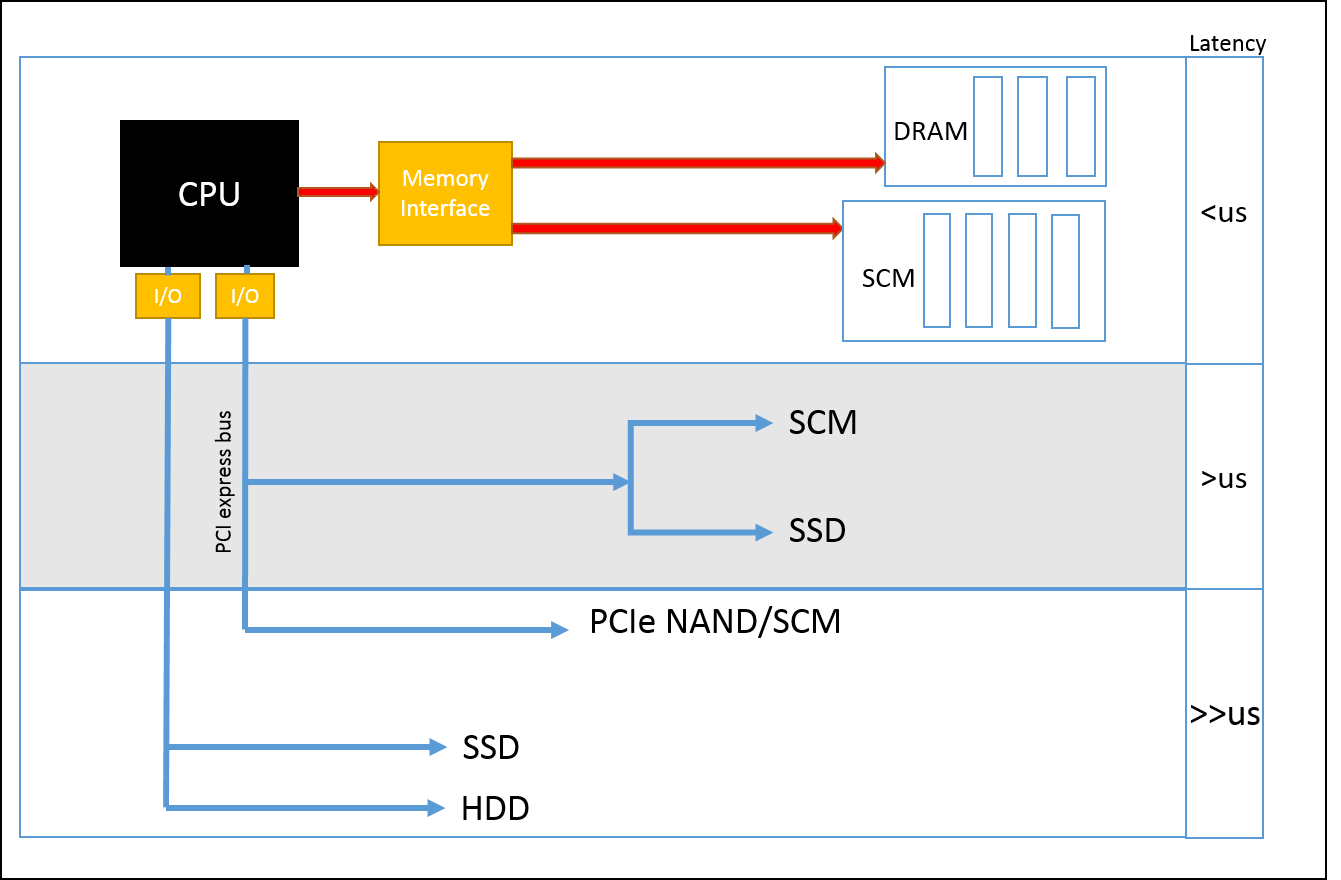
\includegraphics[scale=0.7]{figures/new_mem_arch.png}
  \caption[SCM based Motherboard Architectures]{SCM based Motherboard Architectures \cite{mother_archi}}
  \label{fig:new_arch}
\end{figure}

\subsection{NVDIMM}
Meanwhile another form of Non-volatile RAM in the form of Non-volatile Dual Inline Memory Module (NVDIMM) has become available \cite{nvdimm}. As show in Fig \ref{fig:nvdimm}, it is simply a conventional DRAM backed up by Flash memory. During normal operation all the write and read requests go to DRAM with the flash device remaining inactive. However, in the event of voltage drop (either during normal shutdown, or unexpected power failure) of the power bus, a supercapacitor/battery kicks in to provide alternate power for a short time period. During this time, dedicated hardware logic transfers all the data from DRAM to flash memory, thereby making it non-volatile. The power on procedure restores the state of DRAM from the data backed up in the flash memory. NVDIMMs thus behave exactly like DRAM during runtime, only exposing the flash memory in the reboot sequence. 

\setlength{\belowcaptionskip}{-10pt}

\begin{figure}[H]
  \centering
  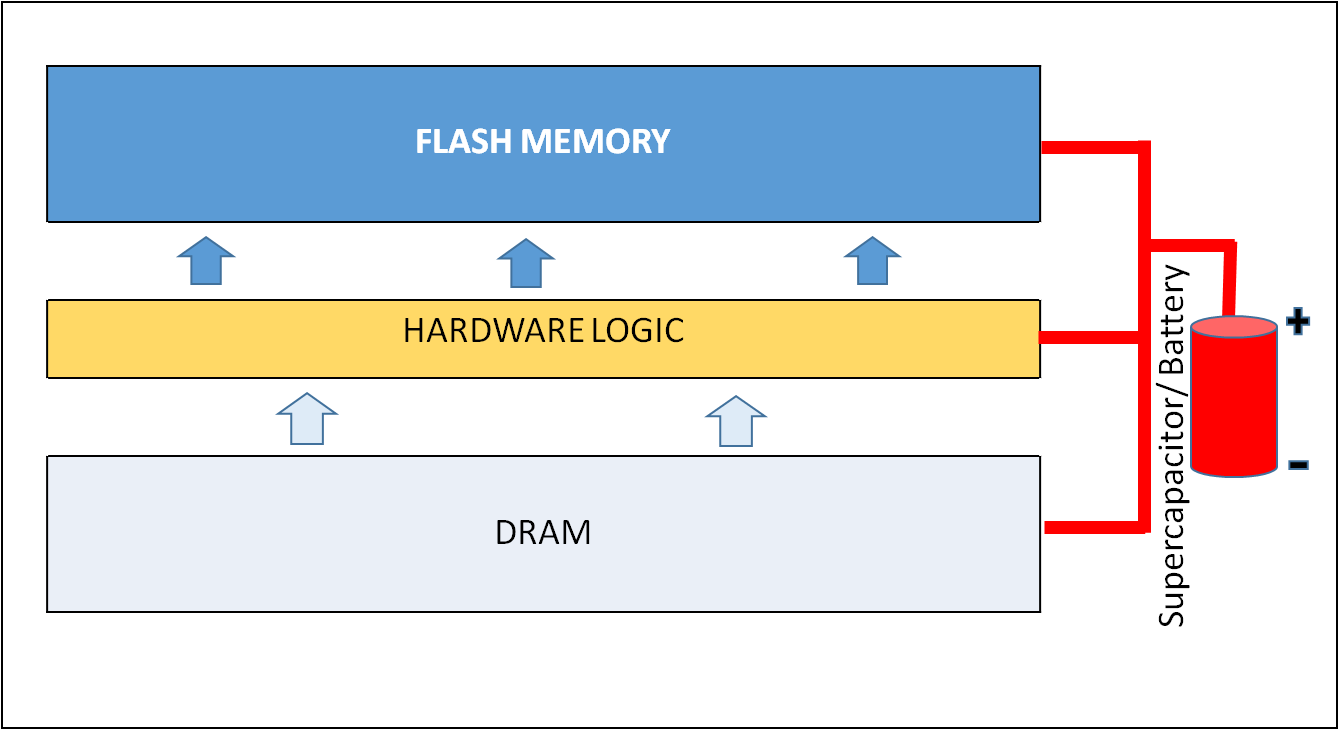
\includegraphics[scale=0.6]{figures/NVDIMM_Stack.png}
  \caption{NVDIMM Model}
  \label{fig:nvdimm}
\end{figure}
One of the key advantages is that NVDIMMs can function at DRAM speeds while providing nonvolatility through background operations. Another important benefit is that both DRAM and flash are commercially mature technologies, combined simply by some hardware glue logic. 

\section{E820 Memory Map}



Devices external to the microprocessor can be broadly classified into two groups

1. I/O

2. Memory

The microprocessor interacts with these two devices in a similar way. I/O devices contain programmable registers, which act as an interface for the device, whereas memory is just a bank of byte addressable memory elements. Both memory and I/O read/write instructions are issued on the same bus, which are then forwarded appropriately by the Northbridge chipset. 

\setlength{\belowcaptionskip}{-10pt}

\begin{figure}[H]
  \centering
  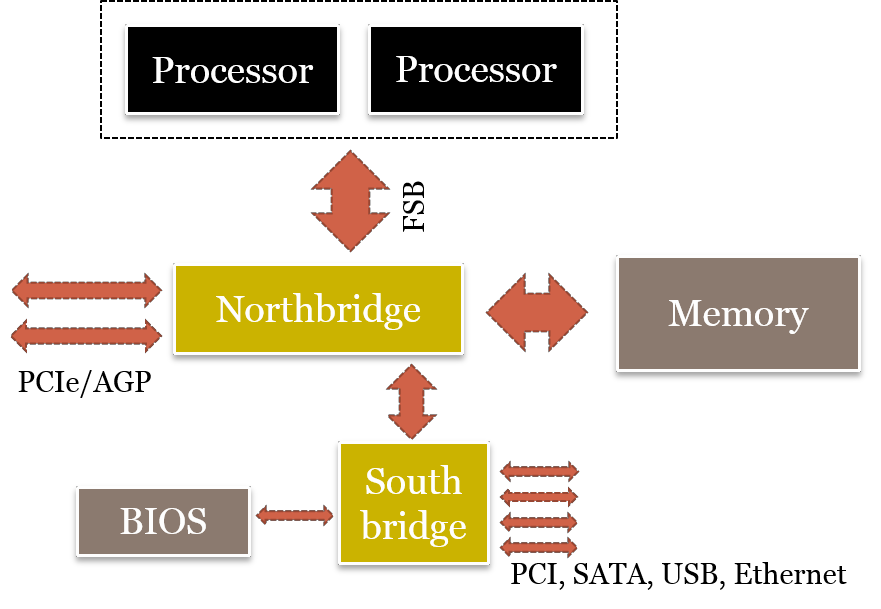
\includegraphics[scale=0.6]{figures/intelhubarchi.png}
  \caption{Intel Hub Architecture}
  \label{fig:intel_arch}
\end{figure}

In the nascent stages of microprocessor development different companies went with different I/O models. Intel included a separate I/O pin in its microprocessor which separated memory and I/O addresses into two separate address spaces, effectively providing an extra bit. For example if the ISA supported 16 bit addresses, we get one 16 bit address space for I/O and another 16 bit address for memory, which is the same as a 17 bit unified address space for both memory and I/O. Intel also had to provide a separate set of I/O instructions to manipulate I/O registers (called I/O ports) in its ISA. This address space segregation through an external I/O pin simplified the address decoding logic in Northbridge chipset. Moreover, then, addresses were just 16 bits wide, making the effective extra bit, a precious resource addition. On the downside, the ISA became more bulky with separate I/O instructions performing similar tasks as Memory instructions.

On the other hand, Motorola provided a Memory Mapped I/O (MMIO) model. Here I/O registers and memory are mapped on to the same address space, each occupying distinct addresses.

This eliminated the need for any separate I/O instructions to be included in the ISA. However, as a result the address decoding logic in the Northbridge chipset became more complex. Where, in the previous case, the chipset just had to check the value of one bit (I/O pin of the microprocessor), here, it had to decode the entire address, to forward the instruction to the correct bus. Moreover this scheme had to share the address space between both memory and I/O.

In the long run, many of the disadvantages of MMIO mentioned above, disappeared, making it the dominant model used in today's computers. With scaling of transistor technology, hardware logic became inexpensive, and the Northbridge could easily handle the additional hardware for complete address decode logic. The address space also expanded from 16 bits to 32 bits and now on to 64 bits, which is more than enough for both memory and I/O. This model had a major advantage of preventing duplication of instructions at the ISA level. The vast plethora of memory management instructions are more comprehensive and can be used in the same way for I/O registers. Thus MMIO is more popular, with I/O ports, only supported for legacy reasons. 

This begs the question now, that how does the OS know the division of the address space between memory and I/O. The translation occurs at Northbridge, and differs from one motherboard to another. These hardware details are hidden in an abstraction layer provided by BIOS (Basic Input/Output System), in the form of E820 Memory Map \cite{acpi_manual}. This list is generated by BIOS on raising a software interrupt 0x15, with EBX set to 0xE820. 

\setlength{\belowcaptionskip}{-10pt}

\begin{table}[H]
  \centering
  %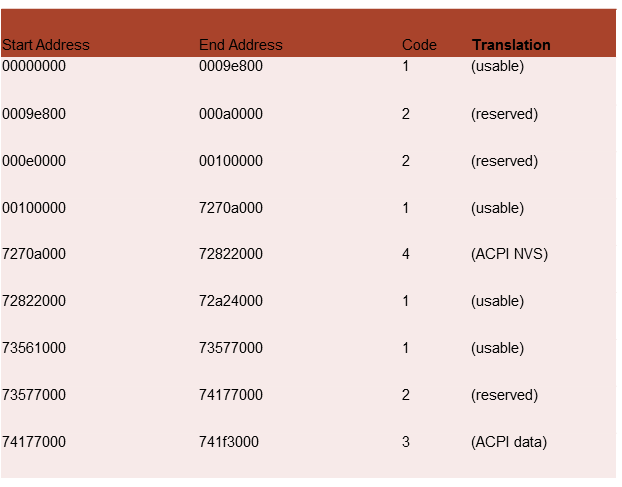
\includegraphics[scale=0.6]{figures/e820table.png}
  \begin{tabular}{|c|c|c|c|}
      \hline
      Start Address & End Address & Code & Translation \\
      \hline 
      \hline
      00000000 & 0009e800 & 1 & (usable) \\
      \hline 
      0009e800 & 000a0000 & 2 & (reserved) \\
      \hline 
      000e0000 & 00100000 & 2 & (reserved) \\
      \hline 
      00100000 & 7270a000 & 1 & (usable) \\
      \hline 
      7270a000 & 72822000 & 4 & (ACPI NVS) \\
      \hline 
      72822000 & 72a24000 & 1 & (usable) \\
      \hline 
      73561000 & 73577000 & 1 & (usable) \\
      \hline 
      73577000 & 74177000 & 2 & (reserved) \\
      \hline
      74177000 & 741f3000 & 3 & (ACPI data)  \\
      \hline
  \end{tabular}
  \caption{Sample E820 Table}
  \label{tab:e820table}
\end{table}



Physical address ranges are currently divided into 6 regions which are indicated by the type field \cite{acpi_manual}.

A brief description of the different types is as follows:

1. AddressRangeMemory: Available RAM

2. AddressRangeReserved: Reserved by the system, generally contains I/O addresses.

3. AddressRangeACPI: Stores ACPI tables.

4. AddressRangeNVS: Not usable by the OS. This range is required to be saved and restored across an NVS sleep.

5. AddressRangeUnusuable: Memory regions containing errors.

6. AddressRangeDisabled: Memory not enabled.

7. Other: Undefined. Reserved for future use.

An E820 memory map contains a list of valid addresses. It serves the following basic services

1. Indicate the physical address space to the OS.

2. Indicating usable RAM regions.

3. Indicate I/O regions, corrupted memory regions, along with other reserved regions.

The first point is very important, since, on boot up the OS is unaware of the amount of memory and I/O devices present in the system. With the knowledge of the memory space the OS can then create page tables and other data structures, to use and share the memory. For the reserved I/O regions, there are several self-discovery mechanisms like Plug and Play (PnP) for devices to identify themselves along with their specific device addresses. 


\section{Intel VT extensions}


Popularity and demand for virtualization led Intel to introduce various features for the x86 platform, in VT-x \cite{intel_manual} and VT-d \cite{intelvtd} extensions. These extensions recognize the following additional modes of operation of the CPU.

1. VMX root: This is the highest level of privilege only accessible to a VMM.

2. VMX non-root: This mode is appropriate for guest VMs, containing all the typical privilege levels encountered by an OS in a non-virtualized environment.

De-privileging an OS relies on extending the traditional framework between applications and OS, to OS and the hypervisor. Sensitive instructions which used to cause traps to the OS, would now trap to the VMX root. These transitions from VMX non-root mode to VMX root mode are termed as VM exits (the reverse is called VM entry). During a VM exit, the state of a guest machine (VM) is saved to, and the state of the host machine (VMM) is restored from, a Virtual Machine Control Structure (VMCS). VMCS is a hardware based memory structure (similar to page table structures) containing various regions defining the CPU state and behavior. It provides a hardware realization to the term vCPU, which was just an abstract concept earlier, realized entirely in software. Since the CPU state is saved to memory by hardware, it is much faster than prior software implementations of storing registers individually. VMCS structures also provide flexibility of masking VM exits on certain sensitive instructions. Interrupts may be remapped to a vCPU, eliminating the need for the VMM to first catch and then deliver these events to guests.

Typically, applications indirectly gain access to system resources via system calls provided by the OS. These system calls were generally implemented using a software interrupt, which would change the privilege level of the CPU and transfer control of execution to a specific OS subroutine. To eliminate the overhead of a software interrupt and allow faster transitioning, Intel added a SYSENTER instruction which would result in a jump to a specified address in the Model-Specific Registers (MSR). A similar functionality has been extended to hypervisors, especially to support paravirtualization. A special VMCALL instruction has been included in the VT-x extensions, which unconditionally causes a VM exit passing the control over to the VMM, in VMX non-root mode. It differs from SYSENTER function in the sense that it stores the guest CPU state to the VMCS structure before moving to the hypervisor, while the SYSENTER instruction does not.

VT-d instructions provide virtualization extensions for devices. It includes facilities such as IOMMU and interrupt remapping which when used in conjunction with VT-x reduce the overhead for I/O operations in virtualized environments. IOMMU has been easier to implement due to the incorporation of northbridge chipset inside the CPU itself. Earlier, memory controllers used to reside on the northbridge chipset external to the CPU. However, due to MOS scaling effects, memory controllers have been moved to the CPU die, and it is a lot easier to support a memory management unit for device memory accesses. VT-d extensions also provide for

interrupt remapping capabilities to vCPUs, rather than physical CPUs further minimizing hypervisor intervention.

These extensions are still an ongoing development, with each revision providing newer features and trying to close the gap between virtualized and non-virtualized environments. Hypervisors are also continually evolving to making extensive use of the added capabilities. 
%%%INCLUDE FIGURES OF COMPUTER MODEL WITH NORTHBRIDGE
